% !TEX root = ../main.tex
% Хавсралт В

\chapter{Ангиллын модулийн нэмэлт үр дүн}
\label{AppendixC}
\pagecolor{white}

Энэ хавсралтын зургуудыг \texttt{appendix\_scripts/gen\_C\_classification.py} script-ээр Туршилт 3-ын \texttt{oof.csv}-аас үүсгэнэ.

\begin{figure}[H]
    \centering
    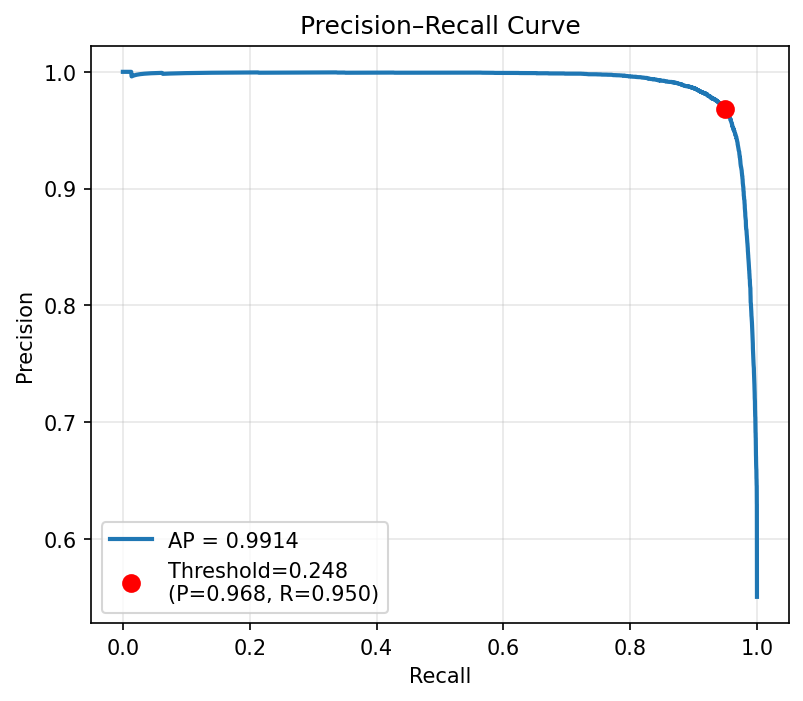
\includegraphics[width=0.58\textwidth,height=0.50\textheight,keepaspectratio]{Figures/appx_c3_pr_curve.png}
    \figcaption{Precision--Recall Curve}{Precision--Recall Curve}
    \label{fig:appC_pr}
\end{figure}

Зураг~\ref{fig:appC_err1}--\ref{fig:appC_err5}-д буруу ангилагдсан жишээнүүдийг үзүүлэв.

\begin{figure}[H]
    \centering
    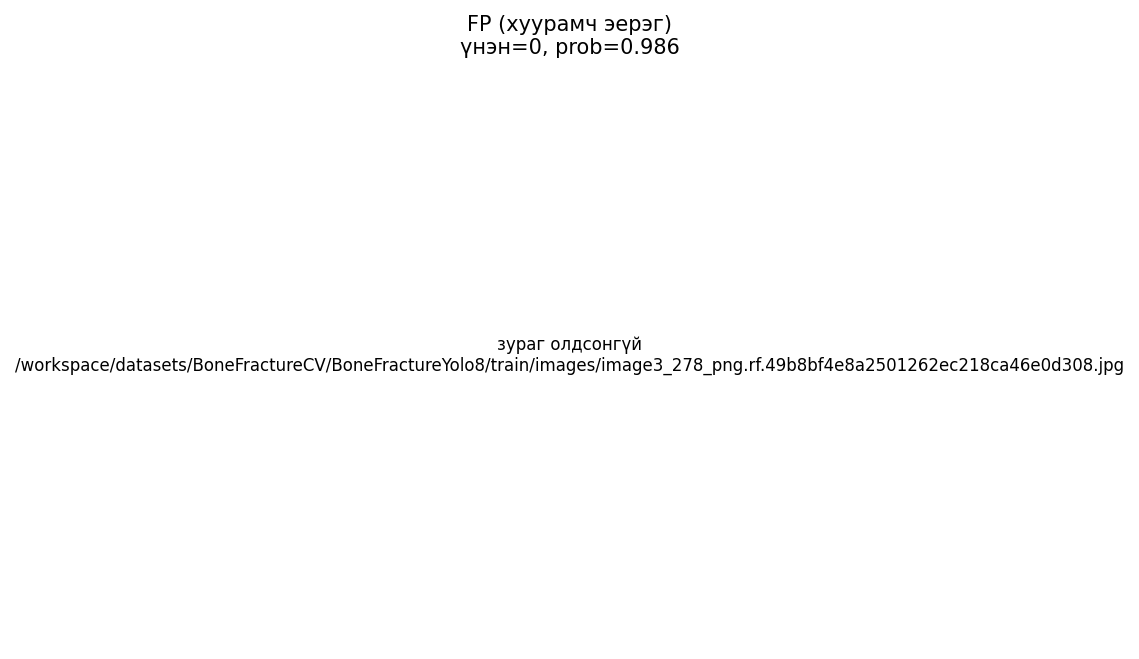
\includegraphics[width=0.62\textwidth,height=0.44\textheight,keepaspectratio]{Figures/appx_c_mis_1.png}
    \figcaption{Буруу ангилагдсан жишээ 1}{Буруу ангилагдсан жишээ 1}
    \label{fig:appC_err1}
\end{figure}

\begin{figure}[H]
    \centering
    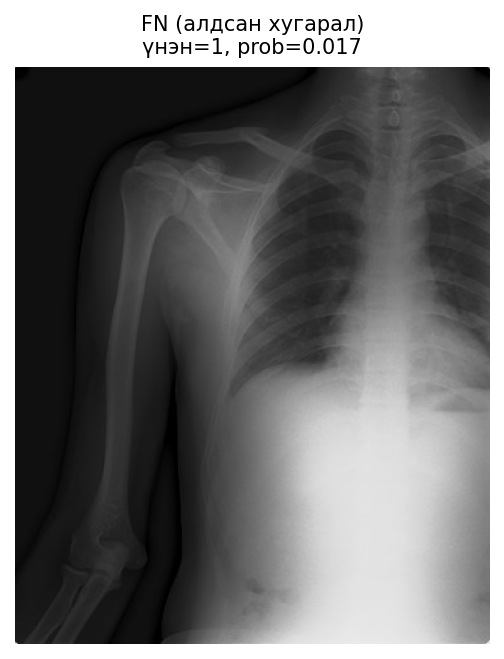
\includegraphics[width=0.42\textwidth,height=0.44\textheight,keepaspectratio]{Figures/appx_c_mis_2.png}
    \figcaption{Буруу ангилагдсан жишээ 2}{Буруу ангилагдсан жишээ 2}
    \label{fig:appC_err2}
\end{figure}

\begin{figure}[H]
    \centering
    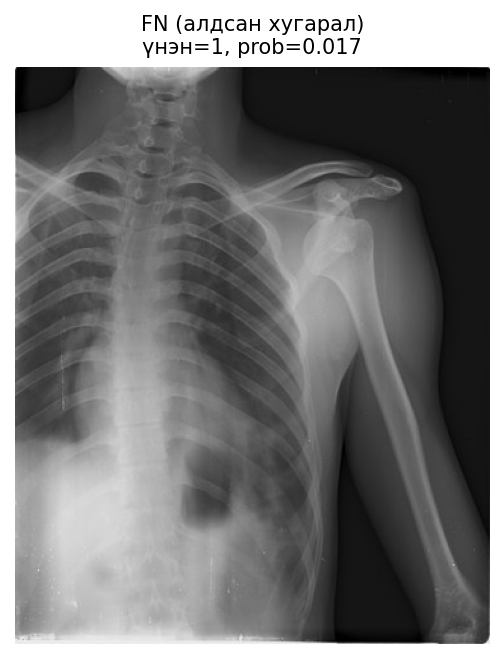
\includegraphics[width=0.42\textwidth,height=0.44\textheight,keepaspectratio]{Figures/appx_c_mis_3.png}
    \figcaption{Буруу ангилагдсан жишээ 3}{Буруу ангилагдсан жишээ 3}
    \label{fig:appC_err3}
\end{figure}

\begin{figure}[H]
    \centering
    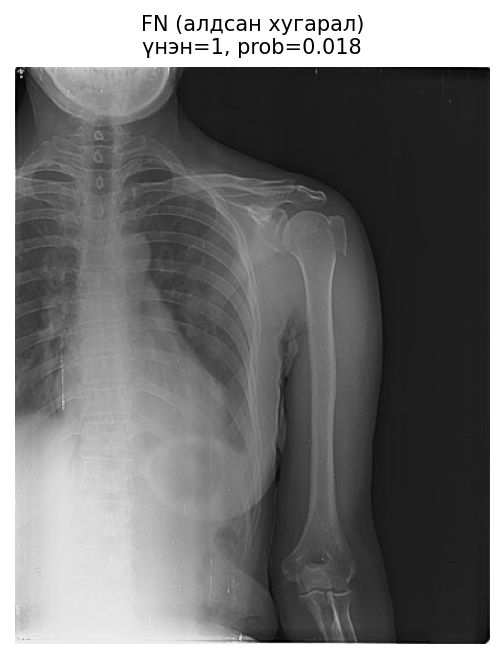
\includegraphics[width=0.42\textwidth,height=0.44\textheight,keepaspectratio]{Figures/appx_c_mis_4.png}
    \figcaption{Буруу ангилагдсан жишээ 4}{Буруу ангилагдсан жишээ 4}
    \label{fig:appC_err4}
\end{figure}

\begin{figure}[H]
    \centering
    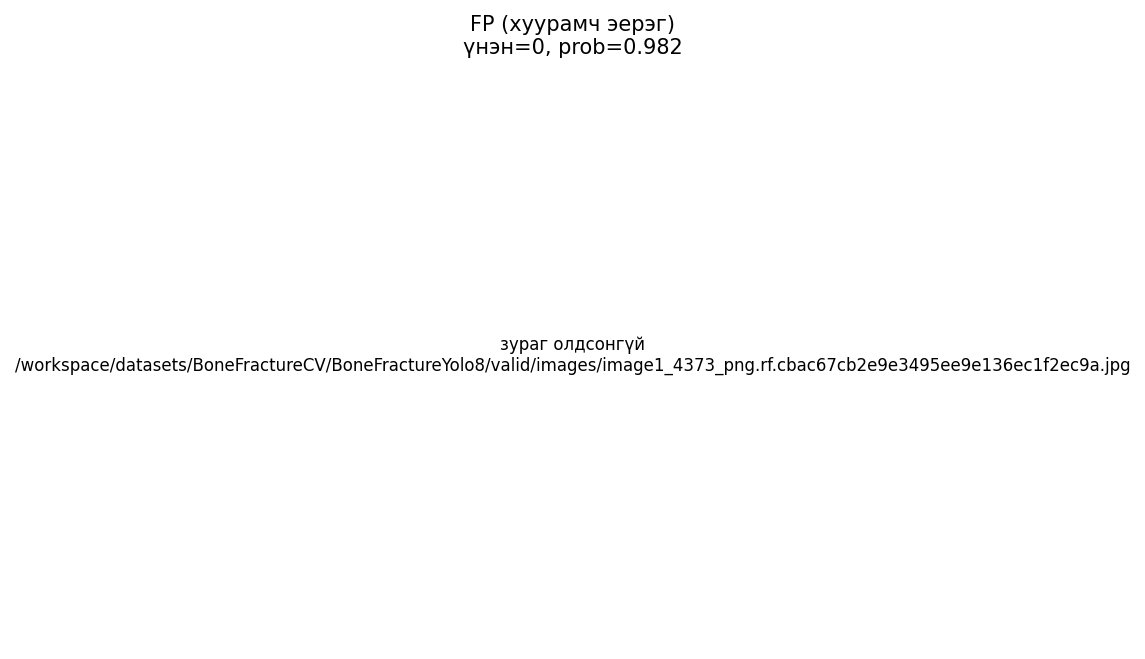
\includegraphics[width=0.62\textwidth,height=0.44\textheight,keepaspectratio]{Figures/appx_c_mis_5.png}
    \figcaption{Буруу ангилагдсан жишээ 5}{Буруу ангилагдсан жишээ 5}
    \label{fig:appC_err5}
\end{figure}

Эдгээр жишээнүүдээс харахад маш нарийн ан цав бүхий болон дүрсний чанар багатай тохиолдлуудад алдаа харьцангуй өндөр ажиглагдсан.
